\documentclass[11pt,a4paper]{report}

\usepackage[utf8]{inputenc}
\usepackage[T1]{fontenc}

\pagestyle{empty}

\usepackage{graphicx} % Include figure files
\usepackage{amstext,amsbsy,amssymb}
%\usepackage{times} 

%% Numbered problems
\newcounter{excount}[chapter]
\newenvironment{exercise}[1][]{\addtocounter{excount}{1} \noindent {\bf Problem
    \arabic{excount} \ \ #1}\hspace{2mm}}{\vspace{4mm}}


\title{FYS3120 Classical Mechanics and Electrodynamics\\ 
\vspace{15mm}Problem set 3}


%%%%%%%
\begin{document}
%%%%%%%
\maketitle


%%%%%%%%
\begin{exercise}
An object with mass $m$ slides without friction on a plane inclined 30$^\circ$. The plane is forced to move horizontally with a constant acceleration $a$. In this case a natural choice of generalized coordinate will be the displacement $s$ of the object along the tilted surface. See Fig.~\ref{fig:incaccplane} for an illustration.

%%%%%%%%%%
\begin{figure}[h]
\begin{center}
\includegraphics[width=6cm]{AkselerertSkraplan.eps}
\end{center}
\caption{Motion on an inclined accelerated plane.}
\label{fig:incaccplane}
\end{figure}
%%%%%%%%%% 

\begin{itemize}
\item[\bf a)] Assume first the inclined plane to be at rest, with vanishing velocity and acceleration. Express the Cartesian coordinates $x,y$ of the sliding object as functions of $s$. Find the Lagrangian expressed in terms of $s$ and $\dot s$.
\item[\bf b)]  Assume next the acceleration $a$ to be constant and non-vanishing. Again find the Cartesian coordinates, and their time derivatives, expressed in terms of $s$ and $\dot s$, and determine the Lagrangian.
\item[\bf c)] Find Lagrange's equation for the system, and solve the equation under the assumption that the body starts at time $t=0$ from the top of the inclined plane ($s=0$) with zero velocity relative to the plane.
\end{itemize}
\end{exercise}
%%%%%%%%%%


%%%%%%%%
\begin{exercise}
A rigid circular metal hoop rotates with constant angular velocity $\omega$ around an axis bisecting the hoop. A particle slides without friction along the hoop and there is no gravity. Use the angle $\theta$ with respect to the rotation axis as generalized coordinate (see Fig.~\ref{fig:hoop}).

%%%%%%%%
\begin{figure}[h!]
\begin{center}
\includegraphics[width=4cm]{RotatingHoop.eps}
\end{center}
\caption{Rotating hoop.}
\label{fig:hoop}
\end{figure}
%%%%%%%%%

\begin{itemize}
\item[\bf a)] Find the Lagrangian expressed in terms of $\theta$ and $\dot\theta$, and derive Lagrange's equation for this variable.
\item[\bf b)] Show that the Lagrangian is the same as the Lagrangian of a particle moving in a time-independent, periodic potential $V(\theta)$, with two stable and two unstable equilibrium points (within a $2\pi$ interval).
\item[\bf c)] With $\theta_0$ as one of the stable equilibrium points, introduce a small deviation, $\phi=\theta-\theta_0$, and determine the small-angle form of the equation of motion (keeping only the lowest order in $\theta$ and its derivative). What is the angular frequency of oscillations about the stationary point?
\end{itemize}
\end{exercise}
%%%%%%%%


%%%%%%%%
\begin{exercise}
Two bodies with the same mass, $m$, are connected with a massless rope through a small hole in a smooth horizontal plane. One body is moving on the plane, the other one is hanging at the end of the rope and can move vertically. At all instances
the rope is tight. The acceleration due to gravity is $g$.

\begin{itemize}
\item[\bf a)] Find Lagrange's equations of motion in polar coordinates ($r,\theta$). 
%and explain their physical meaning. Discuss special cases.
\item[\bf b)] Reduce the equations of motion to a one dimensional problem in $r$ 
%with an effective potential 
and make a qualitative description of the motion. It can be helpful to solve the resulting differential equation numerically.
\end{itemize}

%%%%%%%%%%
\begin{figure}[h!]
\begin{center}
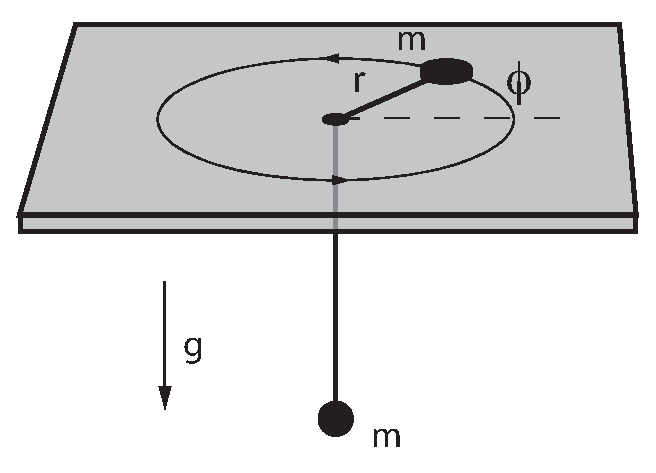
\includegraphics[width=6cm]{KlossOgKule.eps}
\end{center}
\caption{Two bodies connected by a rope through a small hole.}
\end{figure}
%%%%%%%%%%

\end{exercise}
%%%%%%%%


\end{document}

